%!TEX root = ../BoYu-Dissertation.tex
\graphicspath{{Figures/}}

\chapter{Awareness Promotion} % (fold)
\label{cha:awareness_promotion}

% chapter awareness_promotion (end)

\chapter{Designing for Awareness Support} % (fold)
\label{cha:designing_for_awareness_support}
Following the conceptual model of awareness phenomena in complex collaborative activities, we describe the design space of awareness support in this chapter. The goal of this chapter is to identify key design issues to support awareness in distributed, complex collaborative activities, by mapping them to the major components in our conceptual model presented in Chapter \ref{cha:understanding_awareness}. We first present a framework of the whole design space with the major design issues identified. Then we discuss how these design issues have been addressed (or partially addressed) in existing awareness support systems, and the design challenges that motivate our approach. 

\section{The Design Framework} % (fold)
\label{sec:the_design_space}
By conceptualizing the awareness phenomena in distributed, complex collaboration as a continuous development of awareness knowledge (i.e. the knowledge about the environment, activities, and their dependencies) through a variety of cognitive and social processes, the design issues for awareness support can be organized at two levels: the \emph{individual} level and the \emph{team} level. The former focuses on supporting the cognitive processes of individual team members to develop their own awareness, while the latter provides support for the social processes in which team members interact with each other to achieve awareness at the team level. 


\subsection{Designing for individual processes} % (fold)
\label{sub:designing_for_individuals}
At the individual level, the role of computer support can be understood in term of designing `cognitive artifact' \cite{Norman1992}, which is defined as an artificial device designed to maintain, display, or operate upon information in order to aid cognition. Norman argues that an important design consideration for cognitive artifacts is the human action cycle that emphasizes the two sides of human action \cite{Norman1992}. One side is the `evaluation' side of action by perceiving, interpreting and evaluating the state of the environment. The other is the `execution' side that of acting upon the environment. Norman's human action cycle matches well with the major steps of awareness development at the individual level, where the `evaluation' side refers to the \emph{perception}, \emph{comprehension}, and \emph{projection}, and the `execution' side includes the \emph{decision making} and \emph{action execution}.

\subsubsection*{Perception} % (fold)
\label{ssub:perception}

The achievement of individual awareness starts with the ability of individuals to perceive key features in the environment. The primary goal of awareness support in the perception process is to ensure that the awareness information is perceivable to the users. This goal can be achieved from two aspects: \emph{selection} and \emph{presentation} \cite{Berlage1999}. The former focuses on filtering out the information so that only the relevant information is perceived by the users, while the latter involves strengthening the stimulus to ensure that information is perceivable.

\begin{enumerate}
   \item Support for \emph{selection} is based on the assumption that perception is a selective process that depends on the requirements of the current working situation and the tasks at hand \cite{Endsley1995}. Not all information is of relevance to a user, hence the pool of all awareness information has to be processed to filter the relevant information \cite{Berlage1999}. Support for selection is to delegate the effort of filtering out irrelevant information to computer systems, so that human actors can focus on processing only the relevant set of information to avoid information overload.
   \item Support for \emph{presentation} is to strengthen the stimulus in the user interface to ensure important awareness information is perceivable. Existing studies in cognition have shown that the salience of elements in the environment will have a large impact on which portions of the environment are initially attended to, and these elements will form the basis for perception \cite{Hegarty2011}. As a result, the way in which information is presented via the interface will largely influence the perception process by determining which part of the environment will draw the user's attention.
\end{enumerate}

% subsubsection perception (end)

\subsubsection*{Comprehension} % (fold)
\label{ssub:comprehension}
Comprehension is to understand the meaning of perceived awareness information within the context of a user's current goals and activities \cite{oulasvirta2007a}. In the comprehension process, new information must be combined with existing knowledge to develop a composite picture of the situation \cite{Endsley1995}. Hence, the computer support for comprehension is to help the users establish the connection between new awareness information and existing knowledge that forms the inferential framework \cite{carroll2003a}. In general, there are several ways that the comprehension can be supported by computer systems: 

\begin{enumerate}
   \item \emph{Representation}. First, the computer system can support human comprehension by providing external representations of the existing knowledge. Instead of merely relying on the internal representations of human users, the external representation can serve as the information store, so that the internal representation at a given time can be quite sparse, perhaps containing only detailed information about their current focus \cite{Hegarty2011}, or pointers to locations of other important information in the external representation \cite{M.1996}. In this way, the limited working memory resources of human users are freed up for other aspects of cognition \cite{M.1996}.
   \item \emph{Linking}. Second, the computer system can directly aid the linking between new awareness information and existing knowledge by presenting the awareness information along with the contextual information that is potentially relevant to understand its meaning \cite{Tomaszewski2010}. Supporting comprehension by linking has its basis on the design principle of offloading cognitive processes onto perceptual processes \cite{M.1996}. By explicitly linking the awareness information to contextual information for interpretation, some complex cognitive processes, such as searching for and activating the relevant portion of existing knowledge, can be replaced by simple pattern recognition processes \cite{Hegarty2011}. 
\end{enumerate}
% subsubsection comprehension (end)

\subsubsection*{Projection} % (fold)
\label{ssub:projection}
Projection is the process that the individual predicts the future states of other activities based on the comprehension of awareness information. As argued by Endsley \cite{Endsley1995}, this is the most difficult and taxing parts of situation awareness because it requires a fairly well developed mental model of the activities and relationships among them, and the capabilities to perform reasoning. System-generated support for projecting future events and states of the system can then target on supporting the development of the mental model by representing the activities and relationships, or supporting the reasoning processes. 

\begin{enumerate}
   \item \emph{Representation}. Similar to the comprehension process, the projection process can be supported by providing external representations of the existing knowledge to enhance human cognition. However, unlike the representational support for comprehension that focuses on individual activity elements, the knowledge representation for projection emphasizes the various relationships and dependencies among the activity elements, so that the users can infer how the state on one activity can lead to possible changes on other activities' states.
   \item \emph{Reasoning}. The analytical reasoning is central to the projection process, through which users identify possible alternative future scenarios and the signs that one or another of these scenarios is coming to pass \cite{Thomas2006}. As a result, one of the critical requirements for supporting projection is to provide the analytics tools and techniques that allow the users to synthesize information and derive insight from it.
\end{enumerate}

% subsubsection projection (end)
% subsection designing_for_individuals (end)

\subsection{Designing for team processes} % (fold)
\label{sub:designing_for_the_team}
At the team level, the roles of computer in awareness support can be characterized by supporting the three basic types of team processes to propagate awareness information as described in Section \ref{ssub:team_processes}: \emph{feedthrough}, \emph{communication}, and \emph{manifestation}.

\subsubsection*{Feedthrough} % (fold)
\label{ssub:feedthrough}
The process of feedthrough is to make consequences of individual activities apparent to other participants \cite{dourish1992awareness}. In co-located collaborative environments, this usually can be achieved without computer intervention, as collaborators can readily see each other's activities and artifacts they are working on \cite{schmidt2002a}. However, in distributed collaboration, computer support becomes inevitable to enable the process of feedthrough. The role of computer to support feedthrough is to \emph{broadcast} the effects of individual actions and make them visible to each other.
% subsubsection feedthrough (end)
\subsubsection*{Communication} % (fold)
\label{ssub:communication}
Communication is the prevalent form to propagate awareness information, in which people explicitly talk about awareness elements with their collaborators \cite{Gutwin2002}. Computer mediated communication has been an important component in almost every distributed collaborative system, by providing team members a \emph{medium} to communicate with each other remotely.

Although we consider communication as an important process for the team members to propagate awareness information, it is usually supported separately from the awareness systems as a standalone feature in collaborative applications. As a result, we do not put much emphasis on supporting communication in the following discussion.

% subsubsection communication (end)

\subsubsection*{Manifestation} % (fold)
\label{ssub:manifestation}
Manifestation refers to a more subtle means to propagate awareness information among team members. Instead of directly performing actions to impact each other via feedthrough, or explicitly communicating with each other, the team members can make some aspects of their individual awareness visible to others, so that anyone who is interested in these aspects, or who is monitoring the field, can perceive the information. The aspects of individual awareness that can be made visible in the manifestation process can be the raw awareness information perceived by a team member, or his/her interpretation of the awareness information during comprehension/projection, or the results of decision-making. To support the manifestation process, the computer system needs to provide the following functions:

\begin{enumerate}
   \item \emph{Externalization}. The computer system needs to provide the tools to allow the users to externalize aspects of their individual awareness and make them visible to other users.
   \item \emph{Visibility}. The computer system should allow the users to control the visibility of their manifested information. They can specify who can see what piece of the information they make visible.
\end{enumerate}
% subsubsection manifestation (end)
% subsection designing_for_the_team (end)

Table \ref{tab:design_space} summarizes the whole design space with the major design issues for each element identified.

{\footnotesize
   \begin{longtable}{>{\raggedright}m{1.2in}>{\raggedright}p{4.3in}}
\toprule 
\textbf{Awareness Process} & \textbf{Supporting Aspects}\tabularnewline
\midrule 
Perception & \emph{1. Selection}: filtering out the information so that only the
relevant information is perceived by the users

\emph{2. Presentation}: strengthen the stimulus in the user interface
to ensure awareness information is perceivable\tabularnewline
\midrule 
Comprehension & \emph{1. Representation}: providing external representations of the
existing knowledge to support human comprehension

\emph{2. Linking}: presenting the awareness information
along with the contextual information that is potentially relevant
to understand its meaning\tabularnewline
\midrule 
Projection & \emph{1. Representation}: providing external representations of activities
and their relationships 

\emph{2. Reasoning}: provide analytics tools and techniques to help
users perform reasoning\tabularnewline
\midrule 
Feedthrough & \emph{1. }\textit{Broadcasting}: making consequences of individual
activities apparent to other participants\tabularnewline
\midrule 
Communication & \textit{Medium}: providing team members a medium to communicate
with each other remotely\tabularnewline
\midrule 
Manifestation & \textit{1. Externalization}: providing tools for the users to externalize aspects of their individual awareness and make them visible to other users

\textit{2. Visibility}: controlling the visibility of manifested information,
i.e. who can see what piece of the information\tabularnewline
\bottomrule

\caption{Design Space for Awareness Support}
\label{tab:design_space}

\end{longtable}   
}

% section the_design_space (end)

\section{The State of Art} % (fold)
\label{sec:the_state_of_art}
By outlining the design space for awareness support in Section \ref{sec:the_design_space}, we can use it as a framework to review existing studies and awareness systems by looking into how the design aspects in various cognitive and social processes have (or have not) been supported. Before that, we need to make a distinction between two types of awareness models for organizing and processing awareness information: \emph{space-based} and \emph{event-based} models, because it is the underlying awareness model that determines how the awareness processes are supported in an awareness system \cite{Gross2004}.

\subsection{Awareness models} % (fold)
\label{sub:awareness_models}
Most awareness systems rely on certain computational models for organizing and process awareness information. An awareness model usually provides a representation of the field of work, and specifies how awareness information is generated on top of it. In general, we can distinguish two types of awareness models commonly used in existing awareness systems: \emph{space-based} and \emph{event-based} models. 
\subsubsection{Space-based models} % (fold)
\label{ssub:space_based_model}
Many researchers have previously described systems to promote awareness based on the spatial metaphor \cite{Benford1993,Rodden1996,Sandor1997,simone2002a}. These space-based models explicitly represent the field of work as objects (which might represent actors, information, resources, or other computer artifacts) situated and manipulable in some space. Awareness is then achieved by the interaction between actors within the space, as they present themselves and attend to each other in the field \cite{Rodden1996}. Awareness information thus is implicitly embedded as perceivable properties of objects in the space.  

The use of space-based model relies on presenting a `shared space' among collaborators at any given time to provide awareness information, both implicitly and explicitly \cite{dourish1992awareness}. By maintaining the state of the shared work setting, people can either keep an eye on what the rest of the group is doing while doing their individual work, or actively monitor the activities of others, to perceive awareness information \cite{simone2002a}. 

In existing awareness systems, the `shared space' can take different forms \cite{antunes2010a}. 
\begin{enumerate}
   \item `Shared physical space'. In the early work of supporting awareness, a significant effort was devoted to exploring the potential of media space technologies, i.e. an array of continually audio-video links between distributed actors, to provide a `shared physical space' between actors in different locations \cite{Dourish1992}. As with the awareness study, the media space investigations were concerned with informal or social aspect of awareness, and in most cases task-oriented awareness was not mentioned explicitly \cite{schmidt2002a}.
   \item `Shared virtual space'. Rodden \cite{Rodden1996} developed the notion of `virtual space' as a collection of computer-supported interactive spaces. Many collaborative systems offer various types of virtual spaces to support awareness, including abstract media space \cite{Pedersen1997}, virtual meeting rooms \cite{Berlage1999}, and collaborative virtual environment \cite{Benford2001}. Unlike traditional media spaces that aim to establish the `shared physical space', this line of work focuses on the use of abstract representations as awareness indicators. Besides providing a kind of `shielding' for privacy of the people in the shared space \cite{Pedersen1997}, a more interesting feature of using abstract representations is the capability to organize awareness information around task-oriented structures, such as office tables, meeting rooms \cite{Berlage1999}, so that more task-oriented aspects of awareness can be supported.
   \item `Shared workspace'. `Shared workspace' is a specialization of the notion of `shared space' that emphasizes the task-oriented awareness. According to Gutwin and Greenberg \cite{Gutwin2002}, a `shared workspace' is a bounded space where people can see and manipulate artifacts related to their activities. A group editor is a good example of this type of `shared workspace', as it serves to organize activities like writing and revising, while maintaining a coherent view of the whole \cite{dourish1992awareness}. The awareness information in `shared workspace' is presented by attaching it to the manipulable objects through which the task is carried out, and is achieved by user's interaction with the artifacts \cite{Gutwin2002}.
\end{enumerate}
% subsubsection space_based_model (end)

\subsubsection{Event-based models} % (fold)
\label{ssub:event_based_model}
\emph{Event-based} models, on the other hand, provide people with awareness of what is going on around them as expressed by discrete events \cite{rittenbruch2009a}. Each event highlights a piece of awareness information related to certain state change in a collaborative setting for a limited amount of time. Events can be generated by sensors that are associated with actors, shared material, or any other objects that constitute or influence a cooperative environment \cite{prinz1999a}. The list of events that are supported in each awareness system can be totally different, depending on the application domain. As argued by Fuchs et al \cite{Fuchs1995}, we can basically imagine any kind of event, as long as it has a certain relevance when it comes to coordinating the work in a given setting. 

Unlike space-based models where the awareness information is implicitly embedded as properties of objects in the underlying representation of the field of world, awareness information is explicitly represented as first-class objects in event-based models. Each event contains identifiers of the originator, the time, the state change in the collaborative setting, and the context in which the state change took place \cite{fuchs1999a}. Modeling awareness information as first-class objects decouples it from the representation of field of work, which allows the awareness information refers to any change in the field of work, but not necessarily within the user's current viewpoint in the field. The user may attend to their own individual work in the filed, but still be able to receive events about other users that are outside his/her current focus. In this way, the user does not need to monitor the field of work, instead the awareness information is pushed to the user when it becomes relevant.

Because of the decoupling of awareness information from the representation of field of work, many existing event-based systems actually do not need to provide an explicit representation of the field of work \cite{prinz1999a,Fitzpatrick2002}. Even in some systems where the field of work is represented (for example, the GroupDesk \cite{Fuchs1995} and the POLIAwaC systems \cite{sohlenkamp2000po} use semantic networks comprised of actors, artifacts, events, and their relations; the BSBW system \cite{Bentley1995} and Atmosphere model use hierarchical structures of workspaces, to represent the field of work), they are mainly used by the designers to specify events and manage event distributions. 
% subsubsection event_based_model (end)

Table \ref{tab:awareness_models} shows a summary of the major distinguishing features of the \emph{space-based} and \emph{event-based} models. In the following of this section, we will discuss details on how the design aspects in various cognitive and social processes as shown in Section \ref{sec:the_design_space} have (or have not) been supported each of these models.

{\footnotesize
\begin{longtable}{>{\raggedright}p{1.1in}>{\raggedright}p{2.2in}>{\raggedright}p{2.2in}}
\toprule 
 & \textbf{Space-based models} & \textbf{Event-based models}\tabularnewline
\midrule 
\multirow{2}{1.1in}{Field of work} & explicitly represented as a `shared space',  & implementation-dependent representations, \tabularnewline
\cmidrule{2-3} 
 & visible to users & invisible to users\tabularnewline
\midrule 
\multirow{3}{1.1in}{Awareness information} & embedded as perceivable properties of objects in the space & explicitly represented as discrete events\tabularnewline
\cmidrule{2-3} 
 & presented in the context of its origin & can be outside the user's current viewport\tabularnewline
\cmidrule{2-3} 
 & users need to pull the awareness information from the field of work & awareness informaion is pushed to the users\tabularnewline
\midrule 
Example Implementations & 1. physical spaces (e.g. Portholes \cite{Dourish1992})

2. virtual spaces (e.g. AROMA \cite{Pedersen1997},
DIVA \cite{Berlage1999}, MASSIVE-2 \cite{Benford2001})

3. workspaces (e.g. ShrEdit \cite{dourish1992awareness},
GroupKit \cite{Roseman1996}) & GroupDesk \cite{Fuchs1995}, POLIAwaC \cite{sohlenkamp2000po},
NESSIE \cite{prinz1999a}, Elvin \cite{Fitzpatrick2002}\tabularnewline
\bottomrule

\caption{The main distinguishing features of space-based and event-based models}
\label{tab:awareness_models}
\end{longtable}
}
% subsection awareness_models (end)

\subsection{Awareness processes in space-based models} % (fold)
\label{sub:awareness_processes_in_space_based_models}
\subsubsection{Support for perception} % (fold)
\label{ssub:support_for_perception}

\paragraph*{Selection} % (fold)
\label{par:selection}
The first step to support perception regards the selection of the awareness information for a particular user, i.e. what awareness information should be presented? Systems adopting the \emph{space-based} awareness model usually depend on the various relationships between objects inhabiting in the shared space to decide on this.

Benford et al.'s spatial model \cite{Benford1993} provides a formal approach to managing awareness levels between objects inhabiting in a common spatial frame. Awareness between objects is manipulated via \emph{focus} and \emph{nimbus}, two subspaces within which an object chooses to direct either its presence or its attention. Then the awareness information is selected based on the overlapping between the receiver's \emph{focus} and the performer's \emph{nimbus} in certain medium \cite{Benford1993}. Anything about the performer happens in the overlapping area will be perceivable to the receiver. 

The original spatial model has been extended in several ways to support different awareness systems. Sandor et al. \cite{Sandor1997} redefined the concepts of \emph{focus} and \emph{nimbus} upon a semantic network that forms a representation of the working context, and use them to build a generic model `Aether' for supporting awareness in collaborative systems. Rodden \cite{Rodden1996} adopted an object-oriented approach to generalize the spatial model to provide notions of presence, sharing and awareness applicable to applications lacking a spatial metaphor. Simon and Bandini \cite{simone2002a} based on the spatial mode to propose the reaction-diffusion model that can support more user adaptation and dynamic features. Instead of using \emph{focus} and \emph{nimbus}, the awareness information is distributed using field and sensitivity function that allow for a more flexible and compact way of representing various types of nimbi and foci. 

Although various space-based models differ from each other in the specific calculation of awareness levels, the most important point emphasized in all of this work is the insistence that the selection of awareness information is a joint-product between the performer and the receiver, i.e. how the receiver directs the attention to the performer (\emph{focus}) and how the performer projects the presence or activity to the receiver (\emph{nimbus}).
% paragraph selection (end)

\paragraph*{Presentation} % (fold)
\label{par:presentation}
Presenting the awareness information to the user in space-based systems can be achieved in two ways: presenting the information in place of its origin, or presenting in dedicated awareness widgets \cite{Roseman1996}.

As the awareness information is implicitly embedded as properties of objects in the shared spaces, it is natural to present the awareness information directly in place of the associated object in the general presentation of the field of work. For example, in the DIVA shared workspace \cite{Berlage1999}, the color of document icons indicates the document status (e.g. green means `modified by others'). As argued by Dourish and Bellotti \cite{dourish1992awareness}, presenting awareness information in place prevents users from having to switch their attention focus between different information sources. However, this approach relies on the user's capability to perceive and retrieve information from the shared space, which cannot always be guaranteed \cite{Berlage1999}. 

On the other hand, some space-based systems have also explored more lightweight awareness widgets for presenting awareness information \cite{Gutwin1996}. For example, DIVA uses a virtual office table to display participants in a chat room, as well as visualizing their contributions over time\cite{Berlage1999}. The Babble system \cite{Erickson1999} includes a `social proxy' showing team member's level of contribution to a threaded discussion. However, this approach has the major drawback that there is no direct connection between the awareness information and the shared space, which can be disturbing when the user has to switch the focus back forth between the different views. As a result, these lightweight awareness widgets are usually more beneficial for displaying specific aspects of social awareness, such as the collaborator's arrival, availability, involvement, but cannot adequately support task-oriented awareness \cite{carroll2003a}. 
% paragraph presentation (end)
% subsubsection support_for_perception (end)

\subsubsection{Support for comprehension} % (fold)
\label{ssub:support_for_comprehension}
Comparing with event-based systems, support for comprehension can be achieved relatively effortlessly in space-based systems because of two features: the existence of an explicit representation of the shared space, and the possibility of presenting awareness information directly in the shared space. Most existing space-based systems provide visual-spatial displays \cite{Hegarty2011} of the shared spaces, which has a number of advantages to support comprehension. First, they organize information by indexing it spatially. In these displays, space in the display represents space in the field of work, so that if the representation of two items is close in the display, it is likely that those items are also close in the represented field of work. Therefore, information that needs to be related in interpreting and making inferences is likely to be represented by visual features that are close in the display \cite{Hegarty2011}. Second, they provide overviews of the whole field of work, and therefore can be perceived as a whole and provides necessary background for comprehending awareness information \cite{Berlage1999}. Furthermore, as the awareness information can be directly presented in the place of its origin, the user can offload the cognitive effort to locate the related objects onto perceptual processes \cite{M.1996}.

However, space-based systems also have limitations in supporting comprehension. First, we need to distinguish the difference between the context of \emph{origin} of the awareness information and the context of \emph{work} of the user who need to comprehend the information \cite{Gross2004}. Most space-based systems present the awareness information in place of the object where the information occurs on, i.e. within the context of its origin. However, what is more important in the comprehension process is for the user to understand the effects of the awareness information on his/her own work, i.e. within the context of the user's work. Second, the visual-spatial display of the whole field of work can become a difficult or even impractical task when the complexity of the collaboration scales up. When the number of actors, artifacts, and activities increases significantly, such a representation of the whole shared space will also become less efficient to support the comprehension. 
% subsubsection support_for_comprehension (end)
\subsubsection{Support for projection} % (fold)
\label{ssub:support_for_projection}
To our knowledge, explicit support for projection is rarely discussed in existing space-based awareness systems. Most of the space-based systems focus on representing the current state of the `shared space', but how new awareness information will lead to future changes in the `shared space' is usually considered as a cognitive task that is performed by human users. In addition, space-based systems represent the field of work using the spatial metaphor, i.e. the objects are connected based on their spatial relationships in the space. The dependency relationships, which are important knowledge to predict future changes, are not represented.
% subsubsection support_for_projection (end)

\subsubsection{Support for feedthrough} % (fold)
\label{ssub:support_for_feedthrough}
In space-based systems, the process of feedthrough, i.e. making consequences of individual activities apparent to other participants, can be achieved either through the direct video-audio links between actors \cite{Dourish1992}, or through the artifact mediation \cite{Tee2009}. 

In media space-based systems, feedthrough can be supported by the networks of audio and video to provide rich representation of people and their immediate surroundings \cite{Dourish1992}. By seeing others through the media space, it is believed that people can get a sense of others’ activities so that they can infer the consequences of their activities. However, Fish et al.’s study in the use of the Cruiser media space \cite{Fish1992} has shown that even though the media space allows the users to perceive each other's activities, it usually does not provide the visibility of the work artifacts involved in these activities. As a result, showing each other's activities does not necessarily mean the consequences of their activities can be fed through.

As a result, a more common approach to supporting feedthrough in space-based systems is through the common artifacts in the shared spaces, especially in shared virtual spaces and workspace \cite{Berlage1999}. In these systems, users' activities are organized around the common artifacts in the shared spaces. The artifacts provide the awareness information in how they manifest themselves within the space, and in how they provide the group with feedthrough, i.e., when artifacts are manipulated in some activities, they give off information that informs others the consequences of these activities \cite{Tee2009}. However, artifact-mediated feedthrough requires the objects of user's activities can be represented as some artifacts, which may not be applicable in many real world collaboration. For example, the activity of police officers patrolling along the street cannot be easily organized around artifacts.
% subsubsection support_for_feedthrough (end)

\subsubsection{Support for manifestation} % (fold)
\label{ssub:support_for_manifestation}
The basic way to support manifestation in space-based systems is annotations, which are defined as hypertext nodes that are linked to the objects in the shared spaces \cite{Zheng2006,Weng2004}. Annotations allow the users to add their comments or interpretations on specific objects or locations in the shared space that are visible to other collaborators. In this way, annotations provide a way for the users to externalize their individual awareness and display them to others. However, annotations in space-based systems are often bound to the objects in the shared space, and therefore have limited capability to manifest other aspects of individual awareness, such as the intentions to perform activities, or state changes of certain activities. 

Another more sophisticated way to support manifestation has been integrated in the MoMA system in the term of add-on awareness \cite{simone2002a}. The system allows the user to specify field parameters in rule premises to construct add-on awareness promotion. For example, the user can define awareness behavior of the kind: if I receive specific pieces of awareness information, then I will trigger certain interpretation on it, and make the interpretation visible to other actors. The supported manifestation in this way is a reactive process, i.e. actors react to certain changes in the space, however they cannot actively initiate the manifestation process.

% subsubsection support_for_manifestation (end)
% subsection awareness_processes_in_space_based_models (end)

\subsection{Awareness processes in event-based models} % (fold)
\label{sub:awareness_processes_in_event_based_models}
\subsubsection{Support for perception} % (fold)
\label{ssub:support_for_perception}

\paragraph*{Selection} % (fold)
\label{par:selection}
The selection of awareness information in event-based systems focuses on filter out the amount of irrelevant events presented to the users. Many mechanisms that enable the filtering of events have been discussed in the literature, and they vary from each other depending on how the filters are defined. 

\fxwarning{describe the different terms: topic-based, type-based, content-based, etc. so that they can be directly used in later chapter}

In the GroupDesk system \cite{Fuchs1995}, Fuchs et al. define several filters that allowed the limit of the flow of events. On the actor’s side there was an individual privacy filter that allowed the actor to set privacy policies for the events gathered about him. On the perceiver’s side an individual interest filter allowed the perceiver to subscribe only to the events in which he or she was interested. A global filter would allow for the filtering of general conditions (e.g., to comply with organizational policies). Definition of filters in the system is based on individual event types, which consist of a mapping from a set of event types to a list of interested users. The drawback of event type-based filtering is that it requires the user to explicit his/her interest on each event type in a predetermined way, which is a tedious task that the users are not always willing to perform \cite{Grudin1994}. Furthermore, the type-based subscriptions tend to be too rigid or unable to adapt to the team development \cite{Alarcon2002}.

Alternatively, Elvin \cite{Fitzpatrick2002} adopts the content-based filtering of events. It describes events using a set of named attributes of simple data types and consumers subscribe to sets of events using boolean subscription expressions. When a notification is received at the Elvin server from a producer, it is compared to the consumers’ registered subscription expressions and forwarded to those whose expressions it satisfies. A key benefit of content-based notification is the capability to reduce the effort needed to manage event subscription. Instead of subscribing to each type of events, users can subscribe to event patterns, which can describe a set of events. In addition, content-based subscriptions allow the definition of composite events.

ENI \cite{Gross2004} extends the content-based filtering approach and integrates the notion of `contexts' into the model. Context information includes locations, artifacts and applications and other information, which is linked to a specific context. ENI adds this information to existing event information in an awareness system. The model is based on two concepts of context. First, the model tries to determine the context of origin for each event. The authors suggest a context mapping mechanism that maps events gathered from sensor information against rules saved in a context database. Second, the model identifies the work context of the user who is receiving the notification. The work context is derived from the selection of shared workspaces. Based on the two types of context, then the filtering is performed on context matching, i.e. the user defines what types of event context he/she wants to receive in a specific work context. The context-based model tries to improve the event filtering by gathering additional information and allowing users to receive awareness information in a more context-specific manner. However, the context mapping mechanisms underlying this concept is highly complex, and it lacks a formal model to specify the two types of context.

% paragraph selection (end)

\paragraph*{Presentation} % (fold)
\label{par:presentation}
Unlike the \emph{space-based} that relies on the users to monitor the shared space and perceive the presented awareness information, event-based systems make the awareness cues more perceivable for the users than other elements in the environment through different kinds of notification mechanisms \cite{McCrickard2003}. The notification can be done in different ways. In GroupDesk \cite{Fuchs1995} and POLIAwaC \cite{sohlenkamp2000po}, different urgency levels are defined to determine the form of presentation of event information at the user interface. A high urgency would typically lead to a disruptive notification, such as popping up a message window, whereas a low urgency could reflect the information by a change of color of the object's icon and leave the details of information to explicit user request. In NESSIE, the presentation of awareness information is performed by configurable indicators, including simple windows for the listing of event information, different background images, or sounds. Tools are offered that allow the users to easily map awareness events to suitable indicators \cite{prinz1999a}.
% paragraph presentation (end)
% subsubsection support_for_perception (end)

\subsubsection{Support for comprehension} % (fold)
\label{ssub:support_for_comprehension}
Comparing with space-based systems, the comprehension of events provides a more challenging task for the users, as the awareness information is typically presented in separate event-triggered displays peripheral to a person's current task-oriented concern \cite{carroll2003a}. Moreover, event-based systems often do not provide explicit representation of the field of work. As a result, in order for the user to comprehend an event, he/she has to build and maintain a mental model of the inferential framework derived from the field of work, which increases the cognitive load for the user. 

To alleviate this problem, some event-based systems attempt to collocate event notifications within the context of work. For example, NESSIE provides the awareness information by the presentation of pictorial activity indicators for the members of a group as part of the shared workspace user interface \cite{prinz1999a}. In the virtual school project, Carroll et al. suggest that the deadlines and external events should be collocated with process and planning representations \cite{carroll2003a}. However, studies on supporting comprehension of events are still very limited. Questions such as what types of events should be collocated with what types of contextual representations are largely undetermined.  
% subsubsection support_for_comprehension (end)
\subsubsection{Support for projection} % (fold)
\label{ssub:support_for_projection}
Similar to space-based systems, explicit support for projection is rarely discussed in existing event-based awareness systems as well. Most systems assume this as a cognitive task that is performed by human users. 

% subsubsection support_for_projection (end)

\subsubsection{Support for feedthrough} % (fold)
\label{ssub:support_for_feedthrough}
In existing event-based systems, the process of feedthrough can be supported by a specific type of events, i.e. activity events \cite{Fuchs1995}. Activity events are generated by the system. Each time the state of an object changes due to some action of a user, a new event is generated to describe the change. Then the event is sent to the event processing server, and is distributed to the users who subscribe to it. 

% subsubsection support_for_feedthrough (end)

\subsubsection{Support for manifestation} % (fold)
\label{ssub:support_for_manifestation}
Rittenbruch et al. introduce and explore the notion of ``intentionally enriched awareness'' \cite{Rittenbruch2007}, which refers to the process of actively engaging users in the awareness process by enabling them to express intentions. They situate the ``intentionally enriched awareness'' between the event-based awareness systems where actors are not involved at all, and the communication tools where high level of effort from actors is required. This is very similar to our alignment of supporting the three basic awareness propagation processes, and the development of ``intentionally enriched awareness'' can be considered as part of the manifestation process, as it emphasizes the role of actors to make some of their internal states (intentions, reasons, etc.) along with their activities visible to others. Their AnyBiff prototypical system is one of the limited existing attempts to support \emph{manifestation} in awareness systems, which allows users to generate, share, and use a multitude of activity indicators to reveal intentions. The AnyBiff system is mainly used for supporting social awareness in relatively loose-coupled collaborative activities, and hence the information that the users can make visible to each other is very limited. In complex collaborative environments that we are interested in this study, we believe much more aspects of individual awareness could be made visible by the users. Supporting manifestation involves not only help users express their intentions, but also make their interpretations of awareness information during comprehension/projection, or the results of their decision-making visible.
% subsubsection support_for_manifestation (end)
% subsection awareness_processes_in_event_based_models (end)

\subsection{Summary} % (fold)
\label{sub:summary}
Table \ref{tab:awareness_models} shows a comparison of how the major design aspects of supporting awareness processes have been achieved in the \emph{space-based} and \emph{event-based} models.

{\footnotesize
\begin{longtable}{>{\raggedright}p{1.1in}>{\raggedright}p{2.2in}>{\raggedright}p{2.2in}}
\toprule 
\textbf{Awareness Processes} & \textbf{Space-based models} & \textbf{Event-based models}\tabularnewline
\midrule 
Percepetion - Selection & 1. intersections of focus and nimbus that are defined in various forms
\cite{Rodden1996,Sandor1997,Benford1993}

2. comparison of field values agaist sensitivity functions \cite{simone2002a} & 1. type-based filtering \cite{Fuchs1995}

2. content-based filtering \cite{Fitzpatrick2002}

3. context-based filtering \cite{Gross2004}\tabularnewline
\midrule 
Perception - Presentation & 1. in-place presentation \cite{Berlage1999}

2. awareness widgets \cite{Gutwin1996,Erickson1999} & 1. urgency-based notifications \cite{Fuchs1995,sohlenkamp2000po}

2. configurable indicators \cite{prinz1999a}\tabularnewline
\midrule 
Comprehension & 1. visualization of shared spaces

2. direct linking of awaress information to the context of its origin & Collocation event notifications into the display and control of work
objects \cite{prinz1999a,carroll2003a}.\tabularnewline
\midrule 
Projection & rarely supported & rarely supported\tabularnewline
\midrule 
Feedthrough & 1. video-audio links \cite{Dourish1992}

2. artifacts mediated \cite{Tee2009} & Activity event generation and distribution \cite{Fuchs1995}\tabularnewline
\midrule 
Communication & separately supported & separately supported\tabularnewline
\midrule 
Manifestation & 1. annotations \cite{Zheng2006,Weng2004}

2. add-on awareness \cite{simone2002a} & intention-enriched awareness \cite{Rittenbruch2007}\tabularnewline
\bottomrule
\caption{Existing Studies in Awareness Support}
\label{tab:existing_studies}

\end{longtable}
}

Existing systems follow these two types of awareness models have their own pros and cons in supporting awareness processes. 

Space-based models have the advantage that the awareness information is presented in the context of its origin, i.e. the associated object in the shared space, and therefore ease the comprehension process. They relies on the users to monitor the field of work and perceive the awareness information. This can be done efficiently if the local scopes of different users are largely overlapped, as the users can pick up the awareness information peripherally as they work on their own work \cite{schmidt2002a}. However, this becomes much more problematic when the activities of users are distributed and each of them is working on a different set of activities, as actively monitoring the shared space requires extra attentions and efforts from the users. 

On the other hand, event-based models provides a more lightweight way to present awareness information, as only the aspects of awareness information that is of relevance are presented. Furthermore, the event-based presentation is pushed to the users by making the events more perceivable to the users. In this way, the users do not need to switch their attentions to other’s activities until the event notification happens. However, awareness information in the form of events is usually presented separately from the inferential framework to comprehend it, which leads to extra effort in the comprehension process.
% subsection summary (end)
% section the_state_of_art (end)


\section{Discussion} % (fold)
\label{sec:review_discussion}
The major purpose of reviewing existing awareness systems in Section \ref{sec:the_state_of_art} is not to provide an exhaustive evaluation on existing studies. Instead, we use the review to explore design challenges in supporting awareness in complex, distributed geo-collaborative activities that will motivate our approach in the following chapters. 

In general, we can identify two major design challenges based on the analysis in Section \ref{sec:the_state_of_art}.

\textbf{1. The challenge of scaling up.}

Existing systems to support awareness processes are usually designed to support collaborative activities at relatively small and medium scales, it becomes a much more difficult task to support awareness in complex real time activities as we are interested in this study. As we described in Chapter 1, the collaborative activities we consider in this paper are a subset of these complex collaborative setting with two major characteristics: (1) \emph{high level of complexity}: a large number of team workers are geographically distributed in different locations, yet engaged in interdependent activities that require effective coordination. (2) \emph{high level of dynamics}: the actors work in dynamic settings that entail rapid changes in environment and activity, and as a result their specific awareness needs keep changing as the activities are developed.

The two awareness models (\emph{space-based} and \emph{event-based} models) have their own strengths and drawbacks when the collaborative activities scale up. 

On the one hand, \emph{space-based} models manage the awareness through the interaction of collaborators and rely on the users to monitor the field of work and perceive the awareness information. This provides more flexibility to handle increased level of dynamics. As the whole field of work as a shared space is explicitly visible to each user, they can pick up the awareness information relevant to them even when their own interests have been changed. However, space-based models become much more problematic when the level of complexity in the field of work increases. When the number of objects, actors and their activities is significantly increased, the whole field of work will becomes extremely large. Representing the whole field of work and relying on the users to monitor and retrieve awareness information from it becomes a challenging task, as it requires a lot of extra attentions and efforts from the users. 
 
On the other hand, \emph{event-based models} provides a more lightweight way to present awareness information, as only the aspects of awareness information that is of relevance are presented. Furthermore, the event-based presentation is pushed to the users by making the events more perceivable to the users. In this way, the users do not need to switch their attentions to other's activities until the event notification happens. As a result, event-based models can handle more complex situations than space-based models. However, the effectiveness of event-based models largely depends on the quality of event subscriptions, which often requires that considerable domain knowledge be explicitly embedded. As argued by Fuchs et al. \cite{fuchs1999a}, event-based systems seem to work satisfactorily for situations where workflow can be clearly defined in advance or if the application is known from the beginning. When the level of dynamics increases in collaborative activities, such condition can no loner hold. The user's awareness needs are often in the flux of changes, as their activities evolve. Hence, the event-based models becomes less effective in high level of dynamics.

The above analysis clearly shows that neither space-based nor event-based models in existing studies can effectively support awareness processes in collaborative activities when both the complexity and dynamics scale up. Therefore, a new awareness model that can leverage the strengths of both space-based and event-based models becomes extremely important.

\textbf{2. The challenge of integrated support.}

As we conceptualize the awareness phenomena in complex, distributed collaborative activities as a continuous development of awareness knowledge through a variety of integrated cognitive and social processes, it is very important that all the individual and team processes are well supported. However, the review of existing awareness systems shows that some awareness processes have very limited support in existing studies.

At the individual level, existing awareness systems have focused on supporting perception, the higher level of awareness processes are relatively less supported. A possible reason is that the higher-level awareness processes usually involve sophisticated cognitive and reasoning capabilities where the human can do better than the computer. As a result, most awareness systems leave the comprehension and projection to the users. However, in complex collaborative activities, as we discussed earlier, the scaling problem becomes significant, and hence it becomes much more important for the computer to provide functions to amplify and enhance human cognition, not only in the stage of perception, but also in comprehension and projection. 

At the team level, existing awareness systems have focused on either supporting the explicit communication among human collaborators, or different approaches to providing `shared spaces' representing the fields of work so that the actions of each other become visible to each other. However, less discussion has been given to support the awareness interaction via mutual displaying and monitoring, i.e. the manifestation process, which actually is an even more important aspect of awareness in many complex, real world collaborative activities \cite{heath2002a}.

As a result, the second design challenge in supporting awareness in complex collaborative activities is to consider the awareness support from a collective perspective and provide integrated support for the whole awareness development cycle.
% section discussion (end)
% chapter designing_for_awareness_support (end)

\chapter{Overview of Our Approach} % (fold)
\label{cha:our_approach_overview}

Our approach to supporting awareness in complex, distributed geo-collaborative activities aims to address the two major design challenges identified in Section \ref{sec:review_discussion}: 

\begin{enumerate}
   \item As neither space-based nor event-based models in existing studies can effectively support awareness processes in collaborative activities when both the complexity and dynamics scale up, a new awareness model that can leverage the strengths of both space-based and event-based models becomes extremely important.
   \item By conceptualizing the awareness phenomena in complex, distributed collaborative activities as a continuous development of awareness knowledge through a variety of integrated cognitive and social processes, it is very important to consider the awareness support from a collective perspective and provide integrated support for the whole awareness development cycle.
\end{enumerate}

This chapter provides an overview of our approach. The general design principle of our approach is to emphasize the active role of computer system to not merely support, but rather promote awareness in complex collaborative activities. In the following, we first describe the design concept of awareness promotion, and then describe the major components of our awareness promotion framework.

\section{From Awareness Support to Awareness Promotion} % (fold)
\label{sec:from_support_to_promotion}
In order to address the design challenges of scaling up and integrated support, we argue that the computer system needs to play an active role to promote awareness among collaborators. Our awareness promotion approach has its basis in two basic parent disciplines:  artificial intelligence (AI) and human-computer interaction (HCI). 
\begin{enumerate}
   \item From AI, we consider the computer as \emph{an active agent} \cite{Brown99activeuser}, situated within the collaborative environment that adaptively sense, acts, and reacts within this environment over time, to pursue its goal of promoting awareness.
   \item From HCI, we act on the premise that computers and humans have fundamentally asymmetric abilities \cite{Dalal1994}; therefore, we focus on developing divisions of responsibility that exploit the strengths and overcome the weaknesses of both, and utilizing interaction techniques to facilitate effective \emph{human-computer collaboration} \cite{Terveen1995}.
\end{enumerate}

\subsection{The role of computer: from tool to actor} % (fold)
\label{sub:the_role_of_computer}
In existing awareness systems, the role of computer can be described in the metaphor of `tool'. The `tool' perspective emphasizes the human achieves his/her goal through the computer application \cite{Bodker1997}. In term of supporting awareness, it means the human actors use the computer to achieve awareness. The tool perspective emphasizes the control on the human user's side, and how the computer is used to achieve awareness depends on the human user's own knowledge. For example, in space-based systems, the system relies on the user to monitor the shared space to perceive awareness information; in event-based systems, the user needs to explicitly express his/her interests so that the computer can filter out events. 

However, when the collaborative activities become more and more distributed and complicated, more is demanded of the user to control the computer. As we conceptualize the awareness phenomena as a distributed cognitive system (Section \ref{sec:integrated_conceptual_model_of_awareness}), each user usually only have partial knowledge about the whole collaborative situation, and it is unlikely that the user will have the full knowledge of what exactly should be done in order to achieve awareness as a group. The user may have no idea what background information should be attended to in order to interpret a piece of awareness information that is out of his/her local scope of work. Or he/she cannot decide on who should be notified when his/her activities are changed. As a result, the user either uses the partial knowledge to develop awareness that is often incomplete, vague, or even incorrect; or has to extend the mental model to represent more knowledge that out of his/her local scope of work, which inevitably increases the user's cognitive load. 

As a result, we believe that merely relying on the user to control the computer as a `tool' to achieve awareness in distributed, complex collaboration is ineffective. Alternatively, a better approach is to allow the computer to take some control away from the user and actively perform some tasks to help the user to achieve awareness. Instead of relying on the user's internal, partial knowledge to control the awareness development, the computer can maintain a much more complete knowledge representation of the whole field of work at the systematic level, and make use of this knowledge to infer the user's need in the various awareness processes so as to provide awareness support. In this way, the computer can be considered as a `mediator' actively engaged in the collaborative activities along with human actors, but with its own goal (i.e. to assist human actors to achieve awareness), its own mental model (i.e. the knowledge representation of the whole field of work), and its own behaviors (i.e. the capabilities to reason about the user's need in the various awareness processes and adapt interaction and information presentation techniques to support it).
% subsection the_role_of_computer (end)

\subsection{Human computer collaboration} % (fold)
\label{sub:human_computer_collaboration}
While considering the computer as an active actor to support awareness, it does not mean we can delegate all the tasks to the computer and build a completely automatic system. Existing studies in HCI and cognitive science have suggested that the relationship between human users and artificial intelligence should be treated as joint cognitive systems \cite{Dalal1994} or human-computer collaboration systems \cite{Terveen1995}, emphasizing the appropriate partition of responsibility between human actors and computer systems. This perspective of human computer interaction is based on two premises.

\begin{enumerate}
   \item It begins with the premise that computers and humans have fundamentally asymmetric abilities. The computer's strength lies in its ability to store more information than can be stored in the human's short-term memory, to perform faster data retrieval and processing, and to conduct more reliable low-level routine inferences \cite{Brown99activeuser}. On the other hand, the human's strength lies in the ability to integrate information from multiple sources to provide insight necessary to draw complex, higher level inferences, and the capability to handle unexpected situations with the help of long-term memory, experiences, and even intuition. As a result, the goal of computer support is actually to investigate the relationship between the cognitive characteristics of the human and the cognitive characteristics of the computer, and get the computer to complement the human \cite{Dalal1994}.
   \item It assumes that the human and the computer be cooperative to each other in the interaction. It means not only the computer will keep track of the human's activities and adapt its behaviors to support human performance, but also the human is willing to exposing his/her goals and activities to the computer, helping system maintain the knowledge representation, giving away control to the computer, and modifying the computer's behaviors when necessary \cite{Terveen1995}. The goal is not to shield users from the complexities of interaction, but rather to focus on the use of interaction techniques to facilitate effective human-computer collaboration.
\end{enumerate}

In our approach, we also base on these two premises to propose supporting the awareness development in distributed, complex collaboration as a human computer collaborative system. While human actors still need to undergo the cognitive processes to develop individual awareness, and use it to make decision and perform activities in their own local scopes; the computer system take the responsibility to maintain a collective picture of the whole field of work, and utilize this knowledge to facilitate the various cognitive and social awareness processes among human actors.

In sum, we use the term `awareness promotion' to define the paradigm of awareness support that follow these two design principles: (1) the computer plays the role as an `actor' actively engaged in the collaborative activities along with human actors, maintains a collective knowledge representation of the whole field of work, and uses it to adapt behaviors to support the various awareness processes; (2) the computer provides adequate interaction techniques to allow the human actors to collaborate with it to develop awareness at both the individual and team level. 

Table \ref{tab:awareness_support_vs_promotion} illustrates the major differences between the traditional awareness support paradigm and awareness promotion in addressing the different awareness processes. From the table, we can clearly see some of the distinguishing characteristics of awareness promotion. 

\begin{enumerate}
   \item First, the awareness promotion approach emphasizes the computer's knowledge representation of the field of work, and its relationship to awareness information. One one hand, the awareness information is used to update the computer's knowledge representation so that it matches the current state of the field of work. On the other hand, the knowledge representation is used by the computer in almost every awareness process to perform a variety of reasoning tasks to support awareness.
   \item Second, comparing with the traditional awareness support, the awareness promotion approach shows much more frequent interactions between the computer and the human users. Each awareness process involves both the computer's reasoning and the human's cognition, as well as the interaction to combine them together. 
\end{enumerate} 

{\footnotesize
\begin{longtable}{>{\raggedright}p{1.1in}>{\raggedright}p{2.2in}>{\raggedright}p{2.2in}}
\toprule 
\textbf{Awareness processes} & \textbf{Awareness support} & \textbf{Awareness promotion}\tabularnewline
\midrule 
Percepetion & \emph{Space-based} models: 
\begin{itemize}[nosep]
\item the \emph{computer} shares information in a common space
\item the \emph{human} monitors the shared space to perceive information
\end{itemize}
\emph{Event-based} models: 
\begin{itemize}[nosep]
\item the \emph{human} subscribes to events based on interests
\item the \emph{computer} filters out events based on human subscription \end{itemize}
 & \begin{itemize}[nosep]
\item the \emph{computer} uses the information to update its knowlege representation
\item the \emph{computer} uses its knowledge representation to infer who
the information is relevant to, and present it only to the relevant
actors
\item the \emph{user} can modify the computer's knowledge representation \end{itemize}
\tabularnewline
\midrule 
Comprehension & \emph{Space-based} and \emph{event-based} models:
\begin{itemize}[nosep]
\item the \emph{computer} links the awareness information to the context
of its origin
\item the \emph{human} infers the connection between the context of origin
and his/her work context\end{itemize}
 & \begin{itemize}[nosep]
\item the \emph{computer} connects the awareness information to the human's
work context 
\item the \emph{human} interprets the information, and sends the result
to the computer
\item the \emph{computer} updates its knowledge representaton based on human
interpretation\end{itemize}
\tabularnewline
\midrule 
Projection & \emph{Space-based} and \emph{event-based} models:
\begin{itemize}[nosep]
\item the \emph{human} performs the projection on the own\end{itemize}
 & \begin{itemize}[nosep]
\item the \emph{computer} performs the projection based on its knowledge
representation
\item the \emph{computer} presents the projection results to the human
\item the \emph{human} reviews and modifies the computer's reasoning
\item the \emph{computer} updates its knowledge representation based on
human modification\end{itemize}
\tabularnewline
\midrule 
Feedthrough & \emph{Space-based} models:
\begin{itemize}[nosep]
\item the \emph{computer} broadcasts the effect to everyone
\end{itemize}
\emph{Event-based} models:
\begin{itemize}[nosep]
\item the \emph{computer} notified the effect to all subscribers\end{itemize}
 & \begin{itemize}[nosep]
\item the \emph{computer} uses the effect to update its knowlege representation
\item the \emph{computer} uses its knowledge representation to decide on
who should receive the effect and notify them
\item the \emph{human} can control who can see the effects of his/her activities\end{itemize}
\tabularnewline
\midrule 
Manifestation & \emph{Space-based} models: 
\begin{itemize}[nosep]
\item the \emph{human} creates an annotation 
\item the \emph{computer} makes it visible to everyone
\end{itemize}
\emph{Event-based} models:
\begin{itemize}[nosep]
\item the \emph{human} indicates his/her intention as an event
\item the \emph{computer} notified the event to all subscribers\end{itemize}
 & \begin{itemize}[nosep]
\item the \emph{human} generates awareness information indicating some aspects
of his/her individual awareness
\item the \emph{human} can control who can see the generated awareness information
\item the \emph{computer} uses the generated awareness information to update
its knowlege representation
\item the \emph{computer} uses its knowledge representation to decide on
who should receive the information and notify them\end{itemize}
\tabularnewline
\bottomrule
\caption{Awareness support v.s. awareness promotion}
\label{tab:awareness_support_vs_promotion}
\end{longtable}
}

We believe these distinguishing characteristics of awareness promotion approach provide the potential to address the two design challenges, i.e. handling the scaled up complexity and dynamics, and providing integrated awareness support. First, the awareness v approach utilizes the computational knowledge representation to model the field of work and offloads some of the representation and reasoning efforts from the human to the computer. Hence, it can  handle more complex situations than existing awareness models. Meanwhile, the knowledge representation is dynamically updated to reflect the current state of the field of work, which allows it to handle increased level of dynamics. Second, as the computer is equipped with the computational knowledge representation and reasoning capabilities, it allows the computer to provide support on the higher level of awareness processes.
% subsection human_computer_collaboration (end)
% section from_support_to_promotion (end)

\section{The Awareness Promotion Framework} % (fold)
\label{sec:awareness_promotion_framework}
To operationalize the awareness promotion approach, we propose a computational awareness promotion framework. Following our conceptualization of the awareness phenomena in Section \ref{sec:integrated_conceptual_model_of_awareness}, our approach is built on top of two major knowledge components: a computational representation of the field of work based on the SharedPlan theory, and an event-driven model of the awareness processes. Then the computer system's behaviors to promote awareness are embedded in the interaction between these two components. On one hand is how the computer constructs and develops the knowledge representation of the field of work within the event-driven processes, and on the other hand is how the knowledge representation is used to promote these event-driven awareness processes.

This section provides an overview of the awareness promotion framework and discusses the major design choices, but leave the details to the next few chapters.

\subsection{Computational representation of the field of work} % (fold)
\label{sub:computational_representation_of_the_field_of_work}
The nature of awareness phenomena in distributed, complex collaboration as we conceptualized in Section \ref{sec:integrated_conceptual_model_of_awareness}, and the goal of promoting awareness impose several requirements for the knowledge representation of the field of work:

\begin{enumerate}
   \item The knowledge representation should provides a precise model that can capture knowledge about all the three constructs that compose the field of work, i.e. the basic elements of human activities, the local scope of work for each actor, and the various dependency relationships among the activities. 
   \item The knowledge representation should be dynamically updated. Since the awareness needs of users change quickly with the field of work in distributed, complex collaboration, it is essential that the knowledge representation should be kept updating so that it always reflects the current state of the changing field of work.
   \item The knowledge representation needs to be formalized and can be computationally modeled so as to support computer reasoning.
\end{enumerate}

Existing awareness systems have provided several approaches to representing the field of work. The AREA system \cite{fuchs1999a} describes the field of work as semantic networks including relationships among objects, where objects can be human actors artifacts, or aggregations such as groups of people. The representation is primarily used for the users to specify which objects and associated events they are interested in and when they want to be informed. The Atmosphere model \cite{Rittenbruch2002} describes the field of work as a hierarchically structured workspace that consists of a set of \emph{spheres} and \emph{sub-spheres}. Users classify their actions on artifacts by mapping them into different spheres. The MoMA model \cite{simone2002a} applies a reaction-diffusion metaphor to model the field of work as a set of entities embedded in an interaction space, which behave by using diffusion and reaction capabilities. This metaphor is based on the idea that whenever two or more entities have contact, their states are modified in some way. Their states are then propagated to others through fields in the space.  

Although these representations have shown their capabilities to support specific aspects of awareness in their respective application domains, none of them can meet all the three requirements for knowledge representation to enable awareness promotion. The AREA model provides a good representation of the activities and the dependencies using the semantic networks, but the local scopes of each user are not captured. The model is static (as it is pre-determined by the designers), and informal (as it is primarily used as a descriptive framework). The Atmosphere model organizes the field of work around the artifacts without explicit representation of activities. It supports the specification of each user's local scope using private `spheres', but no dependency relationships between activities are supported. It supports the modification to the representation by human users, but the system cannot automatically adapt the representation to changing environment. The MoMA model can support all the three constructs of the field of work as the definition of entities and spaces are generic, and provide some reasoning capabilities. However, it does not support the dynamical adaptation of the model.

In this study we draw knowledge representation and reasoning techniques from existing studies in artificial intelligence to develop a computational model of the field of work that can satisfy all the three requirements. An important feature of our model is the focuses on intentions, beliefs, knowledge, and other attributes of actors' mental states \cite{grosz1996collaborative}. As human actors' awareness processes are directed by their mental models (Section \ref{ssub:individual_processes}), we believe that understanding and representing human actors' mental states allow the computer to infer each actor's local scope, and derive awareness needs from it. We will describe details of the computational representation of the field of work in Chapter \ref{cha:knowledge_reprsentation}, and the dynamic adaptation behaviors in Chapter \ref{cha:knowledge_updating}.
% subsection computational_representation_of_the_field_of_work (end)

\subsection{Event driven awareness processes} % (fold)
\label{sub:event_driven_awareness_processes}
In our approach, we adopt the general event-driven interaction paradigm \cite{Etzion2010} to model the awareness processes. In an event-driven mode of interaction, actors (both human and computer) communicate by generating and receiving events. Each actor receives events from environment and other actors, reacts to them, and generates new events to other actors. We believe that the event-driven paradigm is suitable for modeling awareness processes in our study for two major reasons:

\fxwarning{emphasize the iterative process, the events are connected.}

\begin{enumerate}
   \item The collaborative environments under discussion in this study are naturally centered on events. As we focus on the set of physical collaborative activities that entails rapid and frequent changes in environment and activities, human activities are usually triggered by the detection of events, and then are performed to analyze and react to these events. In the motivating scenario of emergency response, for example, the collective efforts are triggered by an incident, or a disaster, i.e. an event happening in the environment. To respond to the initial event, actors perform activities that add more events building up the situation. In addition, unexpected new events can occur in the environment, requiring continuous response \cite{Turoff2004}. It is these critical events that form the actors' awareness needs and cause the actors to adopt certain goals and perform activities to resolve possible problems.
   \item The event-driven paradigm provides an effective way to represent and process awareness information. Instead of asking the actors to monitor the environment and pull awareness information from it, events are pushed to the actors as they occur. In this way, the actors do not need to split their limited attentions to monitor the environment and each other's activities. This is very important for supporting awareness, as one general design concern for awareness system is that awareness must be achieved with minimal attention and effort so that it does not interrupt the current line of action \cite{schmidt2002a}. 
\end{enumerate}

Our event-driven model of awareness processes shares some commonality with existing event-based models, as both use events as the basic unit to organize and present awareness information. However, they also differ in several important ways:

\begin{enumerate}
   \item In existing event-based models, the computer primarily plays the role as producers of events. It detects events from sensors in the environment or feedbacks of human actions, filters them out based on user subscriptions, and present them to the users. However, in our approach, the computer is also the consumer of events. As to maintain the knowledge representation of the field of work, the computer needs to take the events as input of its reasoning process, and use them to make inference and update its knowledge representation. In this way, the computer behaves like other human actors to consume the events to develop its own awareness.
   \item The concept of events in our approach has a much richer meaning than existing event-based models. It is not only used to describe the occurrences in the environment and in human activities, but also the psychological experience of these occurrences as human actors perceive and interpret them. We make a clear distinction between real world occurrence, event, and awareness in Section \ref{ssub:the_concept_of_events}.
   \item Existing event-based models focus on the generation and presentation of events to the users, but our approach emphasizes the whole process of awareness development driven by events. This means we are not only concerned about how to select and present events to the users, but also how to support the interpretation of these events, and how new events are generated based upon existing ones.
   \fxwarning{the support is not discrete, but continuous.}
\end{enumerate}

In sum, we consider the event not only as a way to represent awareness information, but also an effective interaction mode to drive the awareness development. Each round of awareness development is triggered by receiving certain events, and finished with generating new events that will be consumed by other actors. In the following, we first clarify our concept of event, then describe the event-driven awareness processes. 

\subsubsection{The concept of event} % (fold)
\label{ssub:the_concept_of_events}
Before going further we should clarify what we mean by an event. The concept of the word `event' has been used in the literature from different perspectives:

\begin{enumerate}
   \item The first meaning refers to an actual occurrence (the something that has happened) in the real world. Set out by Quine \cite{quine1985events}, events in this meaning are first-class entities that can be localized in space and time, broken into sub-parts, and arranged in a taxonomic hierarchy. Research using this concept of events primarily focuses on studying the internal structures of the events. For example, in \cite{Yuan2001}, complex geographical phenomena, such as wildfire or precipitation, have been modeled in a hierarchy of events, processes, and states. In \cite{Andrienko2011}, the event-based approach has been adopted to model all the types of occurrences in movement analysis. The focus here is to derive the different event types that may occur and identify the relationships between them.
   \item The second meaning takes us into the realm of computerized event processing, where the word `event' is used to mean a programming entity that represents this occurrence \cite{Spiteri2000}. Each event in this notion is a message that describes an real world occurrence by its source, location, time, and other measurable properties. A single event occurrence can be represented by many event entities, and a given event entity might capture only some of the facets of a particular event occurrence \cite{Etzion2010}.
   \item In event-based awareness systems, the concept of event has a more specific meaning as representing a specific type of awareness information that might be relevant to the user's work. It is usually an application-specific concept, depending on the set of awareness information that is supported by an awareness system. For instance, the AREA system \cite{fuchs1999a} describes events as actions performed on an artifact and the event classes are derived from the artifact class hierarchy and possible operations on them. The ENI system \cite{Gross2004} describes events from the sensors associated with actors, shared artifacts, or any other objects that generate events related to them. 
\end{enumerate}

In this study, we use three different words to avoid the confusion when defining events:
\begin{enumerate}
   \item We use the word \emph{`occurrence'} to denote the real world happenings. It can be in the environment, e.g. the occurrence of a traffic accident at a location; or associated with an object, e.g. a vehicle arrives at the accident spot; or associated with human activities, e.g. the successful performance of first aid on a victim. 
   \item The word \emph{`awareness'} is used to refer to the human consciousness about the occurrences, events, and their relevance to ongoing or future human activities. It emphasizes that awareness is inherently a cognitive, interpretive, and predicative concept that reflects a state of mind.
   \item We use the word \emph{`event'} to denote a computerized entity that describes a piece of awareness information that is relevant to an actor's work. On one hand, it can be the description of a real world \emph{occurrence} by its measurable properties, e.g. the information about a traffic accident with time, location, number of victims etc. On the other hand, it can also be the externalization of an actor's \emph{awareness} knowledge, e.g. an actor's belief that the accident will block the traffic and cause a delay on delivery of medical team.
\end{enumerate}
% subsubsection the_concept_of_event (end)

\subsubsection{Awareness processes} % (fold)
\label{ssub:awareness_processes}
Along with the distinction between the concepts of \emph{`occurrence'}, \emph{`awareness'}, and \emph{`event'} is the notion of dynamic transformations between them (Figure \ref{fig:occurrence_event_awareness}). The transformations are tied to different processes in awareness development. 

\begin{figure}[htbp] %  figure placement: here, top, bottom, or page
   \centering
   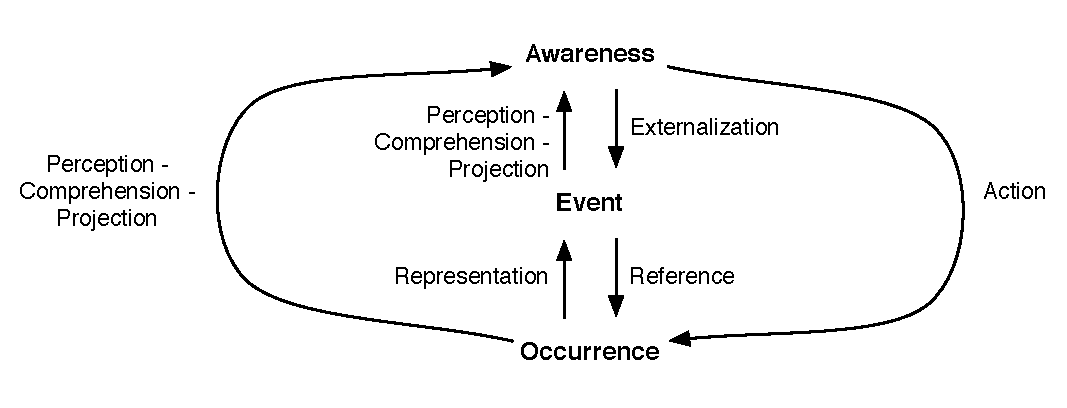
\includegraphics[width=4.5in]{occurrence_event_awareness.pdf} 
   \caption{Transformations between occurrence, event, and awareness}
   \label{fig:occurrence_event_awareness}
\end{figure}

The direct transformation between \emph{occurrence} and \emph{awareness} corresponds to the individual awareness development cycle that has been described in Section \ref{sub:awareness_as_process}. A real world \emph{occurrence} is transformed into \emph{awareness} through an actor's individual awareness processes, i.e. \emph{perception}, \emph{comprehension}, and \emph{projection}. Then, the achieved \emph{awareness} guides the actor's \emph{action} that may generate further \emph{occurrences} in the real world. 

The thing becomes more interesting when the computer support is involved and the transformations are driven by \emph{events}. One one hand is a real world \emph{occurrence} can be captured and represented as an \emph{event} by the computer system, and presented to a human actor. Instead of perceiving the \emph{occurrence} directly, the actor perceives the corresponding \emph{event} in the computer interface, and develops the \emph{awareness} upon it through the actor's individual awareness processes, i.e. \emph{perception}, \emph{comprehension}, and \emph{projection}. On the other hand is some aspect of the actor's \emph{awareness} can be externalized as a new \emph{event}, which refers to some current \emph{occurrence} or predicts future \emph{occurrence} in the real world.

The event-driven transformations can also be used to describe the different awareness propagation processes across multiple actors. The process of \emph{feedthrough} can then be described in the following steps: (1) an actor's \emph{awareness} guides his/her \emph{action} that generates a new \emph{occurrence} in the real world; (2) this new \emph{occurrence} is then captured and represented as an \emph{event} by the computer, and presented to another actor; (3) the other actor develops the \emph{awareness} upon receiving the new event. Similarly, the process of \emph{manifestation} can also be described as follow: (1) an actor's \emph{awareness} is externalized as a new \emph{event}, which refers to some current \emph{occurrence}; (2) this new \emph{event} is then presented to another actor by the computer; (3)the other actor develops the \emph{awareness} upon receiving the new event. 

Figure \ref{fig:example_awareness_traj} shows an example of how these event-driven awareness processes can be combined together to describe a complex trajectory of awareness development that involves three actors in a group. The awareness is propagated from \emph{Actor 1} to \emph{Actor 2} through the process of \emph{manifestation}, and is then propagated from \emph{Actor 2} to \emph{Actor 3} through the process of \emph{feedthrough}.

\begin{figure}[htbp] %  figure placement: here, top, bottom, or page
   \centering
   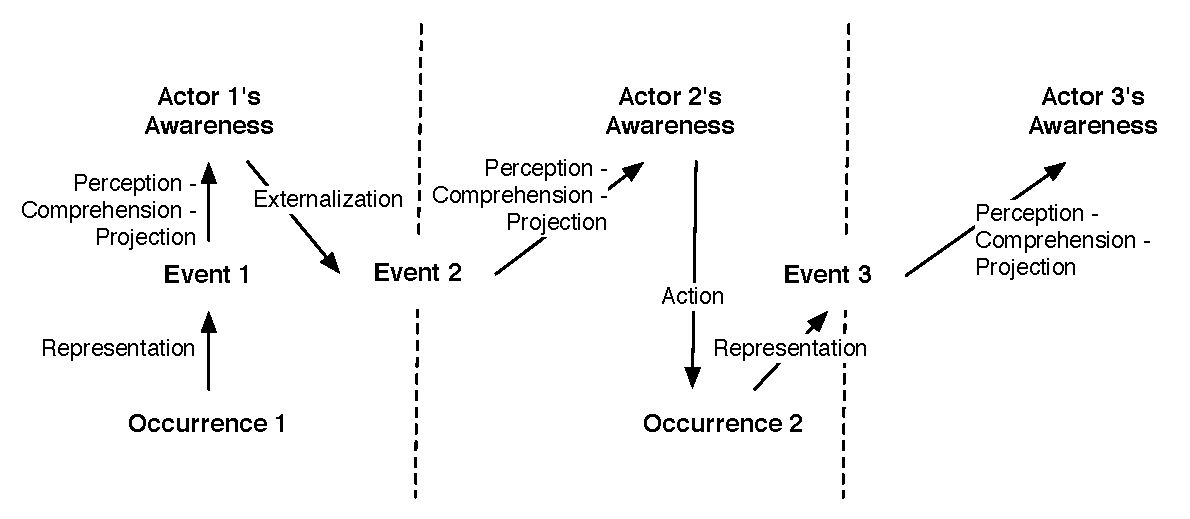
\includegraphics[width=4.5in]{example_awareness_traj.pdf} 
   \caption{An example of event-driven awareness development trajectory}
   \label{fig:example_awareness_traj}
\end{figure}
% subsubsection awareness_processes (end)
% subsection event_driven_awareness_processes (end)

\subsection{The framework} % (fold)
\label{sub:the_awareness_promotion_framework}
Built on top of the computational representation of the field of work, and the event-driven model of the awareness processes, our awareness promotion framework focuses on the interaction between these two components (Figure \ref{fig:awareness_promotion_framework}). 


\begin{figure}[htbp] %  figure placement: here, top, bottom, or page
   \centering
   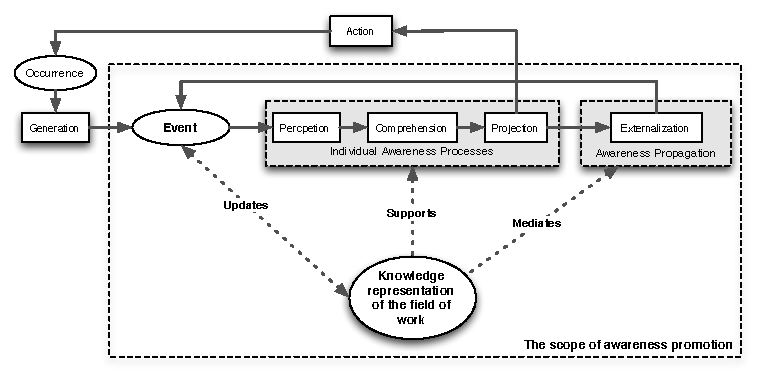
\includegraphics{awareness_promotion_framework.pdf} 
   \caption{Awareness promotion framework}
   \label{fig:awareness_promotion_framework}
\end{figure}

On one hand is how the computer constructs and develops the knowledge representation of the field of work within the event-driven processes. As we argued in Section \ref{sub:computational_representation_of_the_field_of_work}, one of the requirements for the computational representation of the field of work is that it should support dynamic adaptation so that it always reflects the current state of the changing field of work. We utilize the \emph{events} to achieve this goal. As human actors use a subset of the events to develop their individual awareness, the system processes every event to develop its knowledge representation of the whole field of work. The events can be generated by sensing the occurrences in real world, or they can be the results of human actors' externalization of their individual awareness. All of these events will be processed by the computer system to update its knowledge representation of the field of work.

On the other hand, the knowledge representation is used by the computer system to promote the awareness processes. Following the design principle of human-computer collaboration emphasizing the appropriate partition of responsibility between human actors and computer systems (Section \ref{sub:human_computer_collaboration}), the promotion role of the computer system is to strike a balance between the system's reasoning capabilities and providing visual and interactive support. With the computational knowledge about the field of work, the system can offload some of the reasoning effort from the human actors. Meanwhile, the system knowledge can also be visualized to help the human actors perform their part of the work or overwrite the computer's behaviors. 

As shown in Figure \ref{fig:awareness_promotion_framework}, we exclude the event generation process, i.e. the transformation from real world occurrences to events; and the action process, i.e. the transformation from awareness to real world occurrences, from the scope of awareness promotion in this study. It does not mean that these processes are less important or they can be separated from the rest. Rather, we believe these processes are relatively standalone processes that are out of the scope of this study, and therefore we do not claim contributions to these processes. 

The next two chapters provide details of this awareness promotion framework. Chapter \ref{cha:knowledge_reprsentation} describes the two knowledge components, i.e. the computational representation of the field of work and the specification of events, and the mechanisms for updating the knowledge representation with events. Chapter \ref{cha:promoting_event_driven_awareness} describes the promotion of individual awareness processes and awareness propagation.
% subsection the_awareness_promotion_framework (end)
% section awareness_promotion_framework (end)
% chapter our_approach_overview (end)




 

